\chapter{Ngoặc Poisson, các bộ sinh và mômen động lượng}

\lectureoverview{Ngoặc Poisson không chỉ là một cách gọn để viết lại các phương trình Hamilton. Nó là một phép toán đại số sinh ra các phép biến đổi. Lấy ngoặc với Hamiltonian sinh ra sự tiến hóa theo thời gian; lấy ngoặc với động lượng sinh ra các phép tịnh tiến; lấy ngoặc với mômen động lượng sinh ra các phép quay. Trong ngôn ngữ này, đối xứng và bảo toàn trở thành hai cách đọc của cùng một ngoặc bằng không. Chúng ta sẽ phát triển ý tưởng đó từ dao động điều hòa rồi dùng đại số mômen động lượng để thu được tuế sai con quay mà không cần đưa vào các góc Euler.}

\section{Một hàm dọc theo một quỹ đạo Hamilton}

Cho
\[
  F=F(q_1,\ldots,q_n,p_1,\ldots,p_n)
\]
là một hàm khả vi đủ bậc trên không gian pha. Có thể nhìn nó theo hai cách. Thứ nhất, nó gán một số cho mỗi điểm của không gian pha. Thứ hai, một khi đã chọn một quỹ đạo Hamilton, nó trở thành một hàm của thời gian vì điểm \((q(t),p(t))\) di chuyển. Dọc theo quỹ đạo đó,
\begin{equation}
  \frac{dF}{dt}
  =
  \sum_i\left(
    \frac{\partial F}{\partial q_i}\dot q_i
    +\frac{\partial F}{\partial p_i}\dot p_i
  \right).
  \label{eq:l8-chain-rule}
\end{equation}
các phương trình Hamilton,
\begin{equation}
  \dot q_i=\frac{\partial H}{\partial p_i},
  \qquad
  \dot p_i=-\frac{\partial H}{\partial q_i},
  \label{eq:l8-hamilton-equations}
\end{equation}
biến biểu thức này thành
\begin{equation}
  \frac{dF}{dt}
  =
  \sum_i\left(
    \frac{\partial F}{\partial q_i}
    \frac{\partial H}{\partial p_i}
    -
    \frac{\partial F}{\partial p_i}
    \frac{\partial H}{\partial q_i}
  \right).
  \label{eq:l8-fdot-expanded}
\end{equation}
Tổ hợp ở vế phải xuất hiện khắp cơ học cổ điển, ngay cả khi không đối số nào trong hai đối số của nó là Hamiltonian. Điều này gợi ra định nghĩa
\begin{equation}
  \boxed{
  \{F,G\}
  =
  \sum_i\left(
    \frac{\partial F}{\partial q_i}
    \frac{\partial G}{\partial p_i}
    -
    \frac{\partial F}{\partial p_i}
    \frac{\partial G}{\partial q_i}
  \right).}
  \label{eq:l8-poisson-definition}
\end{equation}
Vì thế, phương trình~\eqref{eq:l8-fdot-expanded} là
\begin{equation}
  \boxed{\dot F=\{F,H\}.}
  \label{eq:l8-time-generator}
\end{equation}

\begin{classroomqa}
  \audiencequestion{Nếu thay đối số thứ hai từ \(H\) thành một hàm tùy ý \(G\), thì ngoặc đó vẫn là đạo hàm theo thời gian của \(F\) chứ?
  \lecturetimestamp{00:05:45--00:06:15}}
  \lecturerresponse{Không. Cử tọa đã bắt đúng một điểm quan trọng ngay khi ký hiệu đang được khái quát hóa. Phương trình~\eqref{eq:l8-poisson-definition}
  định nghĩa \(\{F,G\}\) cho mọi cặp hàm trên không gian pha, nhưng
  \(\dot F=\{F,G\}\) chỉ đúng khi \(G\) là Hamiltonian. Một
  \(G\) tổng quát sẽ sinh ra một phép biến đổi vô cùng bé khác.}
\end{classroomqa}

Viết một biến thiên nhỏ theo thời gian dưới dạng
\begin{equation}
  \delta_t F=\epsilon\,\{F,H\}.
  \label{eq:l8-small-time-step}
\end{equation}
là điều hữu ích. Dạng này báo trước điều sẽ đến sau. Sự tiến hóa theo thời gian là một phần tử của một họ lớn hơn các phép biến đổi được sinh ra bởi các ngoặc Poisson.

\section{Đại số của các ngoặc}

Giờ đây có thể dùng ngoặc như một phép tính riêng. Các quy tắc của nó theo từ phép đạo hàm thông thường:
\begin{align}
  \{A,B\}&=-\{B,A\}, \label{eq:l8-antisymmetry}\\
  \{A+B,C\}&=\{A,C\}+\{B,C\}, \label{eq:l8-additivity}\\
  \{\lambda A,B\}&=\lambda\{A,B\},
    \quad \lambda\ \text{constant}, \label{eq:l8-scalar-rule}\\
  \{AB,C\}&=A\{B,C\}+\{A,C\}B. \label{eq:l8-leibniz}
\end{align}
Bốn dòng này lần lượt biểu thị tính phản đối xứng, tính cộng, tính tuyến tính khi nhân với một hằng số và quy tắc Leibniz.
Các hàm cổ điển trên không gian pha nhân với nhau theo tính giao hoán, nên vị trí của các thừa số thông thường \(A\) và \(B\) ở dòng cuối là không quan trọng. Điều đó sẽ không còn đúng đối với các toán tử trong cơ học lượng tử. Tính phản đối xứng cũng suy ra
\begin{equation}
  \{A,A\}=0.
  \label{eq:l8-self-bracket}
\end{equation}

Đối với các tọa độ chính tắc, các ngoặc sơ cấp là
\begin{equation}
  \boxed{
  \{q_i,q_j\}=0,\qquad
  \{p_i,p_j\}=0,\qquad
  \{q_i,p_j\}=\delta_{ij}.}
  \label{eq:l8-canonical-brackets}
\end{equation}
Mọi hàm chỉ phụ thuộc vào các \(q_i\) đều có ngoặc bằng không với mọi hàm khác cũng chỉ phụ thuộc vào các \(q_i\); mệnh đề tương tự đúng cho các hàm chỉ phụ thuộc vào
\(p_i\). Một ngoặc khác không đòi hỏi một tọa độ chính tắc phải ghép cặp với xung lượng liên hợp của nó. Delta Kronecker trong phương trình~\eqref{eq:l8-canonical-brackets} ghi lại rằng chỉ các chỉ số trùng nhau mới ghép cặp.

\subsection{Dao động điều hòa như một phép thử}

Xét
\begin{equation}
  H=\frac{p^2}{2m}+\frac{kq^2}{2}.
  \label{eq:l8-oscillator-hamiltonian}
\end{equation}
Bây giờ ta cố ý chỉ dùng các quy tắc của ngoặc và
phương trình~\eqref{eq:l8-time-generator}. Trước hết,
\begin{align}
  \dot q
  &=\{q,H\}\\
  &=\frac{1}{2m}\{q,p^2\}\\
  &=\frac{1}{2m}\left(p\{q,p\}+\{q,p\}p\right)\\
  &=\frac{p}{m}.
  \label{eq:l8-qdot-oscillator}
\end{align}
Hạng thế năng biến mất vì \(\{q,q^2\}=0\). Tương tự,
\begin{align}
  \dot p
  &=\{p,H\}\\
  &=\frac{k}{2}\{p,q^2\}\\
  &=\frac{k}{2}\left(q\{p,q\}+\{p,q\}q\right)\\
  &=-kq.
  \label{eq:l8-pdot-oscillator}
\end{align}
Dấu trừ này xuất phát đúng từ tính phản đối xứng
\(\{p,q\}=-\{q,p\}=-1\). Kết hợp hai phương trình cấp một này cho
\begin{equation}
  m\ddot q=-kq.
  \label{eq:l8-hooke-equation}
\end{equation}

\begin{figure}[htbp]
  \centering
  
\includegraphics[width=0.82\textwidth]{lecture_08_figure_01.png}
  \caption{Hamiltonian của dao động tử và hai phép tính ngoặc dẫn đến
  \(\dot q=p/m\) và \(\dot p=-kq\).}
  \lectureframe{00:23:20}
\end{figure}

Trong lúc tính toán, cả lớp tìm một động từ mang nghĩa
\emph{take a Poisson bracket} và tạm thời chốt là
\emph{Poissonate}. Câu đùa ấy đánh dấu một sự thay đổi quan điểm có thật: một khi đã biết đại số, ta có thể làm việc trực tiếp với nó thay vì suy ra lại mọi kết quả từ định nghĩa.

\begin{classroomqa}
  \audiencequestion{Cấu trúc toán học này là một nhóm hay một đại số?
  Nó có các phần tử nghịch đảo không? \lecturetimestamp{00:23:48--00:24:16}}
  \lecturerresponse{Nó không phải là một nhóm: phép ngoặc không cung cấp
  phần tử đơn vị và các phần tử nghịch đảo cần có. Các hàm trên không gian pha tạo thành một
  đại số Poisson: chúng có phép nhân và phép cộng giao hoán thông thường,
  cùng với một ngoặc phản đối xứng tuân theo quy tắc Leibniz. Một đồng nhất thức nữa,
  đồng nhất thức Jacobi, hoàn tất định nghĩa trừu tượng thường dùng,
  mặc dù trong bài giảng này không triển khai nó.}
\end{classroomqa}

\begin{classroomqa}
  \audiencequestion{Mối liên hệ giữa ngoặc Poisson và
  giao hoán tử lượng tử là gì? \lecturetimestamp{00:24:18--00:25:00}}
  \lecturerresponse{Bài giảng chỉ đưa ra một sự báo trước. Trong quá trình chuyển sang
  cơ học lượng tử, ngoặc cổ điển được thay thế một cách sơ đồ bởi
  \[
    \{A,B\}_{\mathrm{PB}}
    \longleftrightarrow
    \frac{1}{i\hbar}[\widehat A,\widehat B].
  \]
  Sự tương ứng này đòi hỏi những lưu ý về thứ tự toán tử và
  lượng tử hóa; ở đây nó không được dùng như một định lý.}
\end{classroomqa}

Đối với dao động tử, ngoặc chỉ đơn thuần tái dựng lại các phương trình Hamilton.
Ưu thế thực sự của nó xuất hiện khi phần sinh là một đại lượng bảo toàn khác
\(H\).

\section{Khôi phục mômen động lượng từ đối xứng quay}

Hãy nhớ lại dạng vô cùng bé của cách xây dựng Noether đã dùng trước đó trong khóa học. Nếu một đối xứng liên tục làm thay đổi các tọa độ theo
\begin{equation}
  \delta q_i=\epsilon F_i(q),
  \label{eq:l8-noether-variation}
\end{equation}
thì, trong bối cảnh đang xét ở đây, đại lượng bảo toàn của nó là
\begin{equation}
  G=\sum_i p_iF_i(q).
  \label{eq:l8-noether-charge}
\end{equation}
Thừa số toàn cục \(\epsilon\) có thể được bỏ đi: nhân một đại lượng bảo toàn
với một số cố định không làm thay đổi định luật bảo toàn.

Xét một hạt và quay nó một lượng vô cùng bé quanh trục \(z\). Với quy ước chiều dùng trong bài giảng,
\begin{equation}
  \delta x=-\epsilon y,\qquad
  \delta y=\epsilon x,\qquad
  \delta z=0.
  \label{eq:l8-z-rotation}
\end{equation}
Phương trình~\eqref{eq:l8-noether-charge} cho
\begin{equation}
  L_z=-p_xy+p_yx=xp_y-yp_x.
  \label{eq:l8-lz}
\end{equation}
Hoán vòng \(x\), \(y\) và \(z\),
\begin{equation}
  \boxed{\begin{aligned}
    L_x&=yp_z-zp_y,\\
    L_y&=zp_x-xp_z,\\
    L_z&=xp_y-yp_x.
  \end{aligned}}
  \label{eq:l8-angular-components}
\end{equation}
Đây là các thành phần của
\begin{equation}
  \boldsymbol L=\boldsymbol r\times\boldsymbol p.
  \label{eq:l8-cross-product}
\end{equation}

\begin{figure}[htbp]
  \centering
  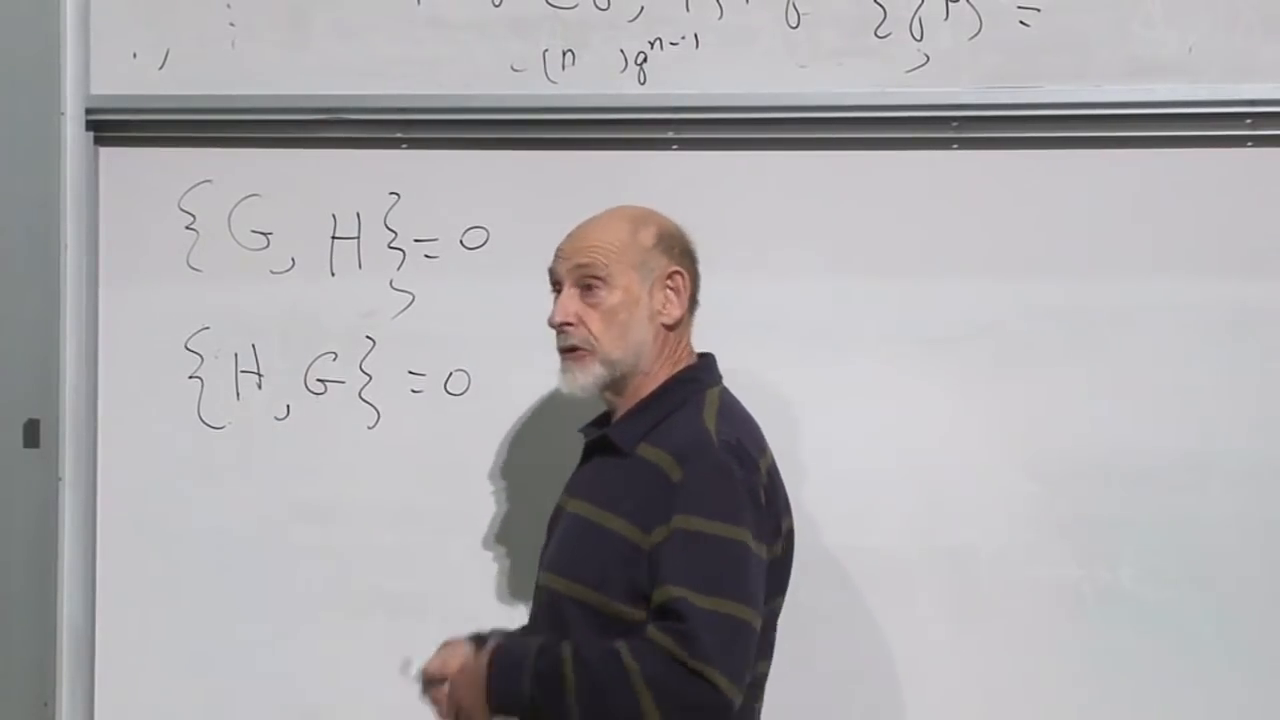
\includegraphics[width=0.82\textwidth]{lecture_08_figure_02.png}
  \caption{Ba thành phần Đề-các của mômen động lượng và dạng tích có hướng gọn của chúng.}
  \lectureframe{00:34:00}
\end{figure}

Phép quay quanh một vectơ đơn vị tùy ý \(\boldsymbol n\) được sinh bởi
\begin{equation}
  L_{\boldsymbol n}=\boldsymbol n\cdot\boldsymbol L.
  \label{eq:l8-arbitrary-axis}
\end{equation}
Đối với một hệ cô lập bất biến quay, cả ba thành phần đều
được bảo toàn. Nếu chỉ còn các phép quay quanh một trục là một đối xứng, thì chỉ
thành phần dọc theo trục đó mới được bảo đảm là bảo toàn.

\section{Mômen động lượng sinh ra các phép quay}

Thay vì lập tức giải một bài toán động lực học quay, hãy khảo sát
\(L_z\) tác dụng thế nào qua ngoặc. Dùng
phương trình~\eqref{eq:l8-lz},
\begin{align}
  \{x,L_z\}
  &=\{x,xp_y-yp_x\}
   =-y\{x,p_x\}
   =-y,\\
  \{y,L_z\}
  &=\{y,xp_y-yp_x\}
   =x\{y,p_y\}
   =x,\\
  \{z,L_z\}&=0.
  \label{eq:l8-position-rotation-brackets}
\end{align}
Đây chính là các hệ số trong
phương trình~\eqref{eq:l8-z-rotation}.

\begin{figure}[htbp]
  \centering
  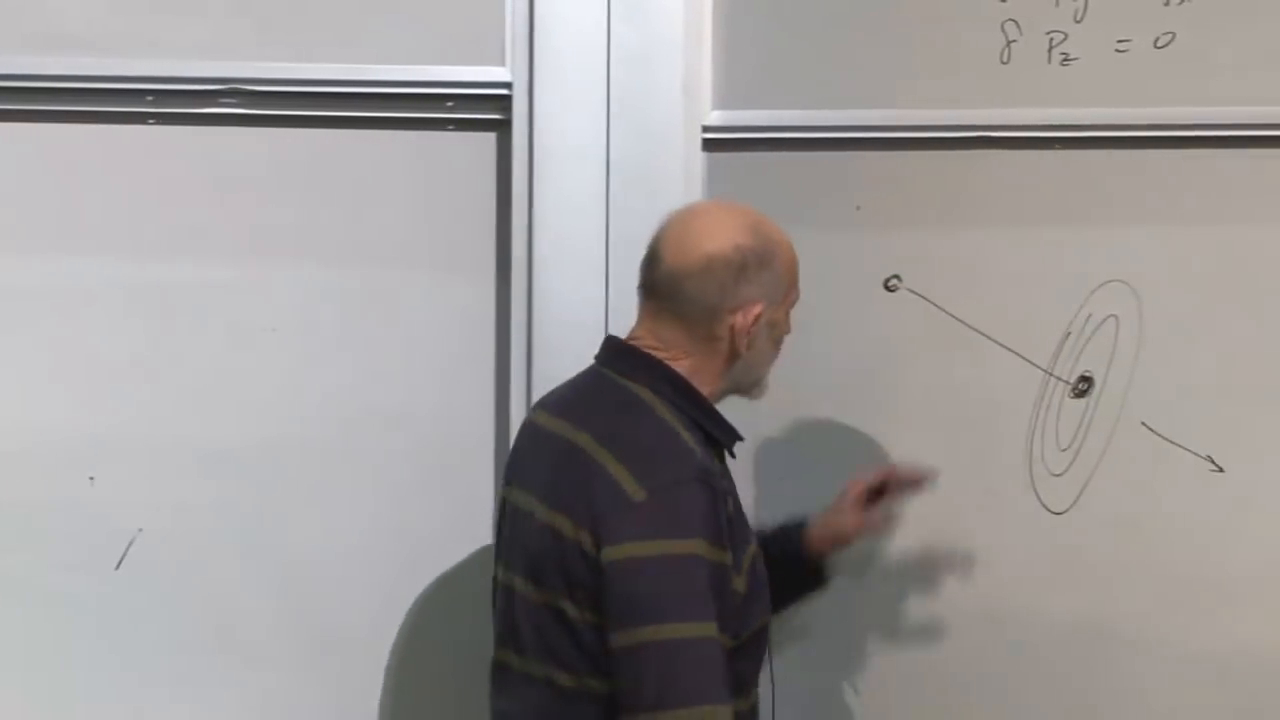
\includegraphics[width=0.82\textwidth]{lecture_08_figure_03.png}
  \caption{Các ngoặc của tọa độ với \(L_z\): ngoặc tái tạo lại
  phép quay vô cùng bé của \((x,y,z)\).}
  \lectureframe{00:38:41}
\end{figure}

Động lượng cũng là một vectơ, và cùng phép tính ấy cho
\begin{equation}
  \begin{aligned}
    \{p_x,L_z\}&=-p_y,\\
    \{p_y,L_z\}&=p_x,\\
    \{p_z,L_z\}&=0.
  \end{aligned}
  \label{eq:l8-momentum-rotation-brackets}
\end{equation}

\begin{figure}[htbp]
  \centering
  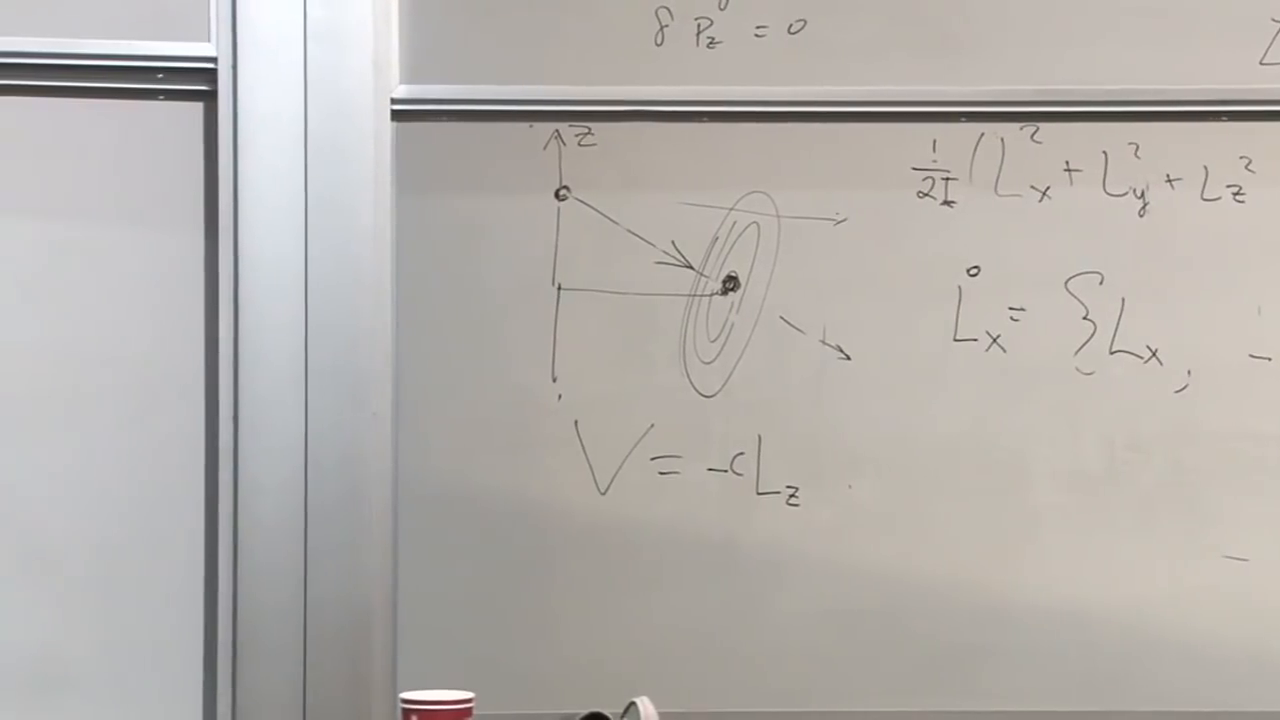
\includegraphics[width=0.82\textwidth]{lecture_08_figure_04.png}
  \caption{Vị trí và động lượng biến đổi theo cùng một mẫu vectơ dưới
  phép quay do \(L_z\) sinh ra.}
  \lectureframe{00:42:08}
\end{figure}

Phát biểu Hamilton tổng quát vì thế là
\begin{equation}
  \boxed{\delta_G A=\epsilon\{A,G\}.}
  \label{eq:l8-generator-rule}
\end{equation}
Mọi hàm trên không gian pha \(G\) đều xác định một phép biến đổi chính tắc
vô cùng bé như thế. Nếu \(G=L_z\), đó là một phép quay. Nếu \(G=H\), đó là một
bước nhỏ theo thời gian.

\begin{classroomqa}
  \audiencequestion{Bài giảng đôi khi nói đến việc quay hệ và đôi khi nói đến việc quay các tọa độ. Quy ước nào được dùng trong các phương trình ngoặc?
  \lecturetimestamp{00:28:22--00:29:35}}
  \lecturerresponse{Phương trình~\eqref{eq:l8-z-rotation} chốt quy ước:
  đó là phép quay chủ động vô cùng bé
  \((x,y)\mapsto(x-\epsilon y,y+\epsilon x)\). Phép quay thụ động của các trục
  mang dấu ngược lại. Một khi quy ước đã được cố định, các công thức ngoặc
  là đơn nghĩa.}
\end{classroomqa}

\section{Động lượng sinh ra các phép tịnh tiến}

Một phép tịnh tiến theo một tọa độ có
\begin{equation}
  \delta q=\epsilon.
  \label{eq:l8-q-translation}
\end{equation}
Ở đây \(F(q)=1\) trong phương trình~\eqref{eq:l8-noether-variation}, nên đại lượng bảo toàn tương ứng
là \(p\). Mệnh đề về phần sinh dự đoán
\begin{equation}
  \{f(q),p\}=\frac{df}{dq}.
  \label{eq:l8-translation-derivative}
\end{equation}
Bài giảng trước hết chứng minh điều này cho lũy thừa bằng quy nạp. Trường hợp cơ sở là
\(\{q,p\}=1\). Giả sử
\begin{equation}
  \{q^{n-1},p\}=(n-1)q^{n-2}.
  \label{eq:l8-induction-hypothesis}
\end{equation}
Khi đó quy tắc tích cho
\begin{align}
  \{q^n,p\}
  &=\{q\,q^{n-1},p\}\\
  &=q\{q^{n-1},p\}+\{q,p\}q^{n-1}\\
  &=(n-1)q^{n-1}+q^{n-1}\\
  &=nq^{n-1}.
  \label{eq:l8-power-translation}
\end{align}
Tính tuyến tính mở rộng kết quả này cho các đa thức và cho các biểu diễn bằng chuỗi lũy thừa hội tụ.
Trực tiếp hơn, định nghĩa của ngoặc cho phương trình~\eqref{eq:l8-translation-derivative} với mọi hàm khả vi \(f(q)\):
\begin{equation}
  \{f(q),p\}
  =
  \frac{\partial f}{\partial q}
  \frac{\partial p}{\partial p}
  =f'(q).
\end{equation}

\begin{figure}[htbp]
  \centering
  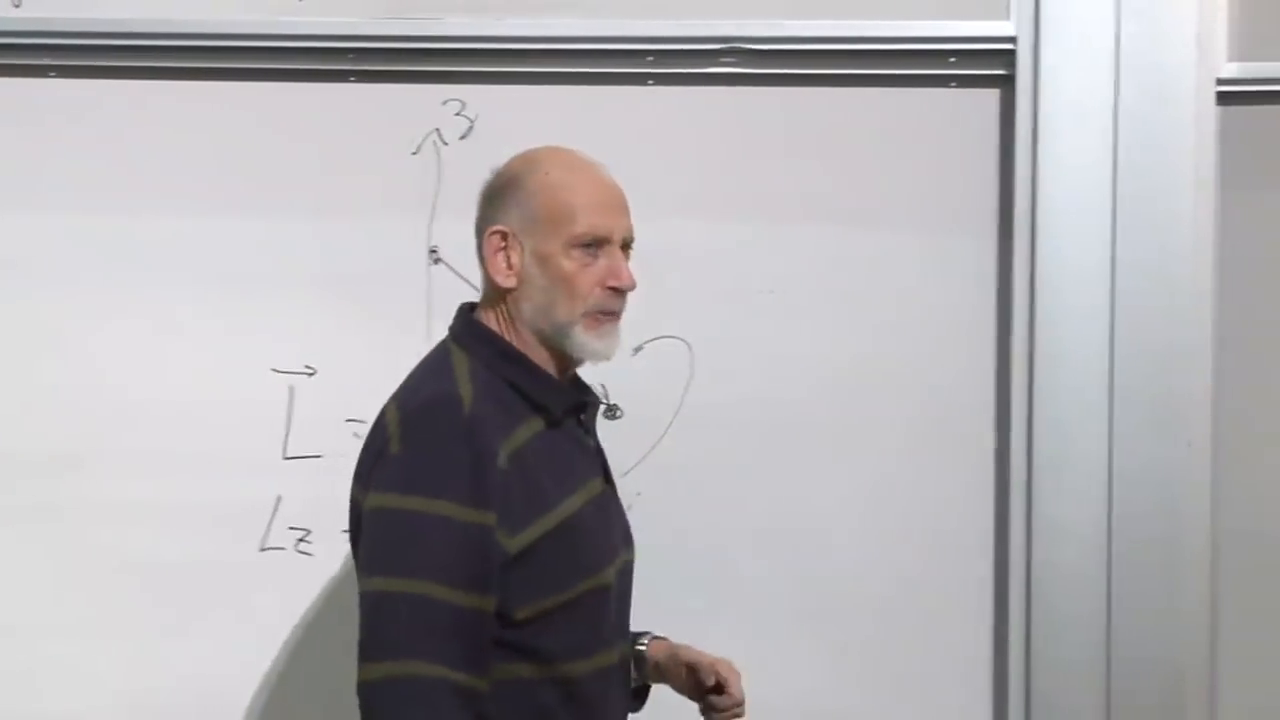
\includegraphics[width=0.82\textwidth]{lecture_08_figure_05.png}
  \caption{Kết quả tịnh tiến sau lập luận quy nạp:
  \(\{F(q),p\}=dF/dq\).}
  \lectureframe{00:53:18}
\end{figure}

Giờ đây ta đã thấy ba phiên bản của một ý tưởng:
\begin{center}
  \begin{tabular}{@{}>{\raggedright\arraybackslash}p{0.37\textwidth}
                      >{\raggedright\arraybackslash}p{0.55\textwidth}@{}}
    \toprule
    Phần sinh và phép biến đổi & Tác dụng vô cùng bé\\
    \midrule
    \(H\), tịnh tiến theo thời gian & \(\delta_tA=\epsilon\{A,H\}\)\\
    \(p_i\), tịnh tiến không gian & \(\delta A=\epsilon\{A,p_i\}\)\\
    \(L_i\), quay & \(\delta A=\epsilon\{A,L_i\}\)\\
    \bottomrule
  \end{tabular}
\end{center}
Đại lượng bảo toàn gắn với một đối xứng liên tục cũng chính là phần sinh của đối xứng đó.

\section{Một ngoặc, hai cách đọc}

Cho \(G(q,p)\) là một phần sinh được đề xuất. Nếu nó được bảo toàn và không có sự phụ thuộc tường minh vào thời gian, thì
\begin{equation}
  \dot G=\{G,H\}=0.
  \label{eq:l8-g-conserved}
\end{equation}
Do tính phản đối xứng,
\begin{equation}
  \{H,G\}=0.
  \label{eq:l8-h-invariant}
\end{equation}
Các phương trình này tương đương về mặt toán học, nhưng cách đọc vật lý của chúng thì khác:
\begin{itemize}
  \item \(\{G,H\}=0\) nói rằng \(G\) không thay đổi dưới sự tiến hóa theo thời gian
  do \(H\) sinh ra.
  \item \(\{H,G\}=0\) nói rằng \(H\) không thay đổi dưới phép biến đổi
  do \(G\) sinh ra.
\end{itemize}
Điều thứ nhất là một định luật bảo toàn; điều thứ hai là một đối xứng của Hamiltonian.
Mối liên hệ của Noether đã được cô đọng vào một số 0.

\begin{figure}[htbp]
  \centering
  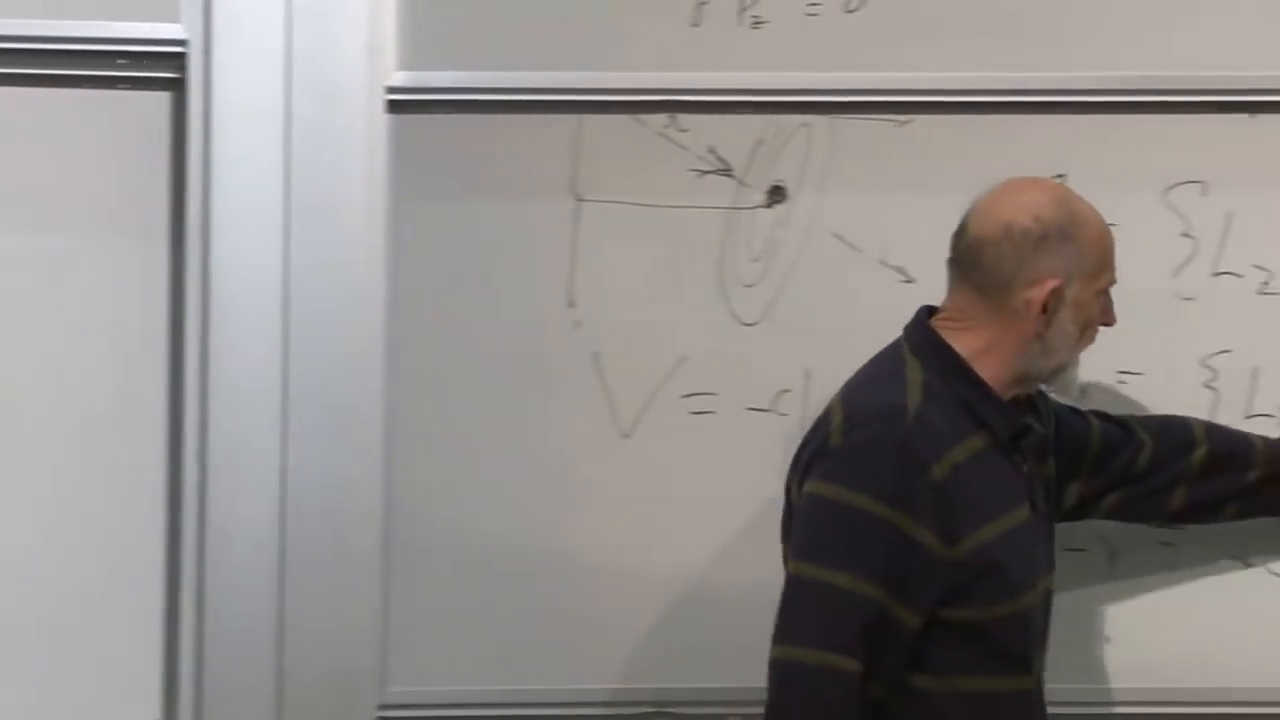
\includegraphics[width=0.82\textwidth]{lecture_08_figure_06.png}
  \caption{Hai thứ tự của cùng một ngoặc bằng không: sự bảo toàn của
  \(G\) và tính bất biến của \(H\) dưới phép biến đổi do \(G\) sinh ra.}
  \lectureframe{01:03:05}
\end{figure}

\begin{classroomqa}
  \audiencequestion{Nếu đã biết một đại lượng bảo toàn, liệu luôn có thể
  khôi phục đối xứng tương ứng không? \lecturetimestamp{01:01:42--01:02:15}}
  \lecturerresponse{Trong khuôn khổ Hamilton này, có: lấy ngoặc mọi
  biến trên không gian pha với \(G\). Toàn bộ các quan hệ
  \(\delta_GA=\epsilon\{A,G\}\) cho biết các biến biến đổi như thế nào. Chẳng
  hạn, các ngoặc với \(L_z\) cho thấy một phép quay ngay cả khi cách
  diễn giải đó chưa được biết trước. Những điểm tinh tế toàn cục và biên
  có thể xuất hiện trong các bối cảnh nâng cao hơn, nhưng phát biểu địa phương vô cùng bé
  là điều được dùng ở đây.}
\end{classroomqa}

\begin{classroomqa}
  \audiencequestion{Những phương trình ngoặc đó có cho ta biết chuyển động vật lý
  đứng sau định luật bảo toàn không?
  \lecturetimestamp{00:56:01--00:58:13}}
  \lecturerresponse{Không. Chúng xác định phép biến đổi đối xứng, chứ không phải
  quỹ đạo thực sự. Sự bảo toàn của \(L_z\) cho biết có đối xứng quay;
  nó không nói rằng hạt chuyển động theo một đường tròn. Sự tiến hóa theo thời gian thực sự
  được sinh bởi \(H\). Một ngoặc với phần sinh khác mô tả một
  hướng biến đổi khác trong không gian pha.}
\end{classroomqa}

\begin{classroomqa}
  \audiencequestion{Có một phát biểu tổng quát về phép biến đổi nào không,
  mà không giả sử sẵn tính bảo toàn? \lecturetimestamp{01:02:40--01:04:45}}
  \lecturerresponse{Có. Phương trình~\eqref{eq:l8-generator-rule} xác định một
  phép biến đổi vô cùng bé cho mọi hàm \(G\), bất kể nó có được
  bảo toàn hay không. Nó chỉ trở thành một đối xứng khi Hamiltonian bất biến:
  \(\{H,G\}=0\). Cùng điều kiện ấy, đọc theo thứ tự ngược lại, khi đó nói
  rằng \(G\) được bảo toàn.}
\end{classroomqa}

\section{Đại số mômen động lượng}

Phép tính tiếp theo cho phép ta không còn phải mang các tọa độ của hạt theo trong
mọi bài toán quay. Bắt đầu với
\[
  L_x=yp_z-zp_y,\qquad
  L_z=xp_y-yp_x.
\]
Trong \(\{L_x,L_z\}\), phần lớn các hạng chéo triệt tiêu vì các chỉ số của chúng không tạo thành
các cặp chính tắc. Các phép co còn lại cho
\begin{align}
  \{L_x,L_z\}
  &=\{yp_z-zp_y,xp_y-yp_x\}\\
  &=xp_z-zp_x\\
  &=-L_y.
  \label{eq:l8-lx-lz}
\end{align}
Đảo thứ tự thì dấu trừ biến mất. Hoán vòng các tọa độ cho
\begin{equation}
  \boxed{\begin{aligned}
    \{L_x,L_y\}&=L_z,\\
    \{L_y,L_z\}&=L_x,\\
    \{L_z,L_x\}&=L_y.
  \end{aligned}}
  \label{eq:l8-angular-algebra}
\end{equation}
Theo ký hiệu chỉ số,
\begin{equation}
  \{L_i,L_j\}=\varepsilon_{ijk}L_k.
  \label{eq:l8-angular-algebra-index}
\end{equation}

\begin{figure}[htbp]
  \centering
  \includegraphics[width=0.82\textwidth]{lecture_08_figure_07.png}
  \caption{Đại số ngoặc Poisson theo chu kỳ của ba thành phần mômen động lượng.}
  \lectureframe{01:10:52}
\end{figure}

Kết quả này cũng có thể đã được dự đoán trước. Vì \(\boldsymbol L\) là một vectơ, lấy ngoặc thành phần \(x\) của nó với \(L_z\) phải cho biến thiên vô cùng nhỏ của thành phần ấy dưới một phép quay quanh \(z\), tức là \(-L_y\). Phép tính tường minh xác nhận lập luận hình học đó. Các phương trình này cũng là tiền thân cổ điển của các hệ thức giao hoán mômen động lượng lượng tử.

\section{Con quay hồi chuyển quay nhanh}

Xét như một ứng dụng, ta xét một con quay hồi chuyển: một bánh đà quay rất nhanh có tâm cách điểm tựa một khoảng cố định \(R\). Gọi \(\boldsymbol r\) là vectơ hướng từ điểm tựa tới tâm bánh. Bánh đà quay quanh trục của nó nhanh đến mức mômen động lượng trội của nó vẫn thẳng hàng với hướng ấy. Trong gần đúng được dùng trong bài giảng,
\begin{equation}
  \boldsymbol L=\ell\,\boldsymbol r,
  \qquad
  L_z=\ell z,
  \label{eq:l8-L-parallel-r}
\end{equation}
trong đó \(\ell=L/R\) được xem là hằng số. Ban đầu bỏ qua các mômen động lượng nhỏ hơn gắn với chương động hoặc chuyển động của trục.

\begin{figure}[htbp]
  \centering
  \begin{tikzpicture}[scale=0.95,>=Latex]
    \coordinate (P) at (0,3.2);
    \coordinate (C) at (3.7,1.55);
    \draw[->] (0,-0.2) -- (0,4.35) node[above] {\(z\)};
    \fill (P) circle (1.7pt) node[left] {pivot};
    \draw[very thick,->] (P) -- (C)
      node[midway,above right] {\(\boldsymbol r\parallel\boldsymbol L\)};
    \fill (C) circle (1.7pt);
    \draw[dashed] (P) -- (0,1.55);
    \draw[dashed] (0,1.55) -- (C);
    \node[left] at (0,1.55) {\(z\)};
    \begin{scope}[shift={(C)},rotate=-24]
      \draw[very thick] (0,0) ellipse (0.65 and 1.35);
      \draw[thick] (0,0) ellipse (0.42 and 0.9);
    \end{scope}
    \draw[->,thick] (2.15,2.85)
      arc[start angle=140,end angle=35,radius=1.65];
  \end{tikzpicture}
  \caption{Gần đúng con quay nhanh. Khoảng cách từ điểm tựa đến tâm là cố định, và mômen động lượng tự quay trội vẫn thẳng hàng với trục và \(\boldsymbol r\).}
\end{figure}

\begin{figure}[htbp]
  \centering
  \includegraphics[width=0.82\textwidth]{lecture_08_figure_08.png}
  \caption{Hình phác trên bảng của bánh đà cùng với
  \(H_{\rm rot}=L^2/(2I)\) và sự triệt tiêu chứng minh rằng \(\boldsymbol L\) được bảo toàn
  khi không có mômen lực.}
  \lectureframe{01:18:54}
\end{figure}

\subsection{Không có trọng lực: vì sao mọi thành phần đều giữ nguyên}

Đối với rôto đối xứng trục đã được đơn giản hóa,
\begin{equation}
  H_{\mathrm{rot}}
  =\frac{1}{2I}
  \left(L_x^2+L_y^2+L_z^2\right)
  =\frac{L^2}{2I}.
  \label{eq:l8-rotational-hamiltonian}
\end{equation}
Hệ số là \(1/(2I)\), không phải \(I/2\); sự nhầm lẫn đó đã xuất hiện rồi được sửa trên bảng. Dùng phương trình~\eqref{eq:l8-angular-algebra},
\begin{align}
  \dot L_x
  &=\{L_x,H_{\mathrm{rot}}\}\\
  &=\frac{1}{2I}\left(
    2L_y\{L_x,L_y\}
    +2L_z\{L_x,L_z\}
  \right)\\
  &=\frac{1}{I}\left(L_yL_z-L_zL_y\right)=0.
  \label{eq:l8-free-lx}
\end{align}
Theo phép hoán vị vòng,
\begin{equation}
  \dot L_x=\dot L_y=\dot L_z=0.
  \label{eq:l8-free-angular-momentum}
\end{equation}
Đại lượng vô hướng \(L^2\) có ngoặc bằng không với từng thành phần \(L_i\); theo ngôn ngữ của đại số này, nó là một Casimir. Vì vậy, một con quay hồi chuyển không chịu mômen lực giữ nguyên cả độ lớn lẫn hướng của mômen động lượng của nó.

\begin{classroomqa}
  \audiencequestion{Ở đây mômen quán tính chỉ là một con số thôi sao?
  \lecturetimestamp{01:14:23--01:15:05}}
  \lecturerresponse{Với mô hình rút gọn này thì đúng vậy. Nó mã hóa sự phân bố khối lượng của bánh quanh trục quay của nó. Một vật rắn tổng quát có tensor mômen quán tính và một Hamilton quay
  \(\sum_i L_i^2/(2I_i)\) trong các trục chính. Bài giảng chọn rôto nhanh, đối xứng đơn giản hơn vì mục tiêu là trình bày phương pháp ngoặc Poisson chứ không phải phát triển đầy đủ động lực học vật rắn.}
\end{classroomqa}

\subsection{Trọng lực và dấu của thế năng}

Lấy tọa độ thẳng đứng \(z\) dương theo chiều lên trên và đặt điểm tựa tại gốc tọa độ. Thế năng hấp dẫn của tâm bánh là
\begin{equation}
  V=Mgz.
  \label{eq:l8-mgz}
\end{equation}
Vì \(L_z=\ell z\),
\begin{equation}
  V=cL_z,
  \qquad
  c=\frac{Mg}{\ell}=\frac{MgR}{L}.
  \label{eq:l8-potential-lz}
\end{equation}
Ở đây \(c>0\) khi \(\boldsymbol L\) được chọn cùng hướng với
\(\boldsymbol r\). Nếu bánh đà quay theo chiều ngược lại, quan hệ có dấu giữa \(\boldsymbol L\) và \(\boldsymbol r\) đảo ngược, và tần số tiến động có dấu tương ứng cũng đảo ngược.

\begin{figure}[htbp]
  \centering
  \includegraphics[width=0.82\textwidth]{lecture_08_figure_09.png}
  \caption{Hình học với độ dài cố định làm cơ sở cho
  \(\boldsymbol L=\ell\boldsymbol r\) và \(L_z=\ell z\).}
  \lectureframe{01:25:38}
\end{figure}

\begin{figure}[htbp]
  \centering
  \includegraphics[width=0.82\textwidth]{lecture_08_figure_10.png}
  \caption{Một trạng thái trung gian trên bảng cho thấy \(V=-cL_z\). Dấu này
  được sửa về sau sau khi \(z\) được cố định là hướng lên trên: với
  \(\boldsymbol L=\ell\boldsymbol r\) và \(\ell>0\), kết quả nhất quán là
  \(V=+cL_z\).}
  \lectureframe{01:22:43}
\end{figure}

\begin{classroomqa}
  \audiencequestion{Vì sao có thể thay độ cao bằng một thành phần của mômen động lượng? Đường xiên đó là một trục hay một vectơ vị trí?
  \lecturetimestamp{01:22:20--01:25:43}}
  \lecturerresponse{Đường xiên đó tốt nhất nên được ký hiệu là
  \(\boldsymbol r\), vectơ từ điểm tựa cố định đến tâm bánh. Một trục vật lý có thể nằm dọc theo nó, nhưng quan hệ được dùng trong phép tính là
  gần đúng quay nhanh \(\boldsymbol L=\ell\boldsymbol r\). Vì thế, các thành phần \(z\) của chúng
  tỉ lệ với nhau. Cuộc trao đổi trực tiếp đã đổi nhãn vài lần trước khi
  chốt lại sự phân biệt này.}
\end{classroomqa}

\begin{classroomqa}
  \audiencequestion{Những giả thiết nào làm cho \(\ell\) là hằng số, và điều gì không còn đúng nếu tâm bánh có thể trượt theo phương bán kính?
  \lecturetimestamp{01:25:43--01:26:38,\allowbreak\ 01:34:22--01:35:00}}
  \lecturerresponse{Tự quay trội được giả sử lớn hơn nhiều so với mômen động lượng
  gắn với chuyển động chậm, và khoảng cách từ điểm tựa đến tâm
  là cố định. Khi đó độ lớn spin thay đổi rất ít và
  \(\boldsymbol L\) quay cùng với \(\boldsymbol r\). Nếu tâm có thể trượt
  theo phương bán kính, \(z\) sẽ không còn tỉ lệ với \(L_z\) bằng một hệ số hằng
  duy nhất, nên Hamilton rút gọn \(V=cL_z\) sẽ không mô tả được chuyển
  động.}
\end{classroomqa}

\begin{classroomqa}
  \audiencequestion{Tại sao trên bảng lúc đầu là dấu trừ và về sau lại là dấu cộng? Chiều spin có quan trọng không?
  \lecturetimestamp{01:27:13--01:28:15,\allowbreak\ 01:33:09--01:33:21}}
  \lecturerresponse{Dấu ban đầu là một lỗi viết trực tiếp trên bảng trộn lẫn với một
  quy ước trục chưa ổn định. Khi \(z\) đã được định nghĩa là hướng lên trên,
  \(V=Mgz\) tăng theo độ cao. Nếu
  \(\boldsymbol L=\ell\boldsymbol r\) với \(\ell>0\), điều này cho
  \(V=+cL_z\). Đảo chiều spin sẽ đảo ngược tính tỉ lệ có dấu và
  hướng tiến động, nhưng không khôi phục được một lựa chọn dấu tùy ý.}
\end{classroomqa}

\subsection{Tiến động từ ba phương trình ngắn}

Hamiltonian rút gọn đầy đủ là
\begin{equation}
  H=
  \frac{1}{2I}\left(L_x^2+L_y^2+L_z^2\right)+cL_z.
  \label{eq:l8-full-gyro-hamiltonian}
\end{equation}
Ta đã chỉ ra rằng \(L^2\) có ngoặc bằng không với mọi \(L_i\). Chỉ hạng tuyến tính đóng góp:
\begin{align}
  \dot L_z&=\{L_z,H\}=0,\\
  \dot L_x&=\{L_x,H\}=c\{L_x,L_z\}=-cL_y,\\
  \dot L_y&=\{L_y,H\}=c\{L_y,L_z\}=cL_x.
  \label{eq:l8-precession-equations}
\end{align}

\begin{figure}[htbp]
  \centering
  \includegraphics[width=0.82\textwidth]{lecture_08_figure_11.png}
  \caption{Các phương trình thành phần cuối cùng: \(L_z\) không đổi, còn
  \(L_x\) và \(L_y\) quay vào nhau.}
  \lectureframe{01:30:35}
\end{figure}

Thành phần thẳng đứng và độ lớn nằm ngang là hằng số:
\begin{equation}
  \frac{d}{dt}(L_x^2+L_y^2)
  =2L_x(-cL_y)+2L_y(cL_x)=0.
\end{equation}
Gộp các thành phần nằm ngang,
\begin{equation}
  L_+=L_x+iL_y,
  \qquad
  \dot L_+=icL_+,
\end{equation}
nên
\begin{equation}
  L_+(t)=L_+(0)e^{ict}.
  \label{eq:l8-precession-solution}
\end{equation}
Vì vậy vectơ mômen động lượng tiến động quanh trục thẳng đứng với tốc độ góc \(|c|=MgR/L\). Độ nghiêng của nó vẫn giữ cố định trong chuyển động đều lý tưởng hóa này.

\begin{classroomqa}
  \audiencequestion{Hạng năng lượng quay có bị bỏ qua khi viết các phương trình tiến động không?
  \lecturetimestamp{01:35:01--01:35:49}}
  \lecturerresponse{Không. Nó thuộc Hamiltonian đầy đủ như trong
  phương trình~\eqref{eq:l8-full-gyro-hamiltonian}. Nó chỉ đơn giản đóng góp bằng không vào
  \(\dot L_i\) vì \(\{L_i,L^2\}=0\), một sự triệt tiêu đã được chứng minh trong phép tính
  không có mômen lực. Câu hỏi của sinh viên làm cho bước ngầm này trở nên
  tường minh.}
\end{classroomqa}

\begin{classroomqa}
  \audiencequestion{Tiến động đều có phải là một trạng thái cân bằng không? Điều gì xảy ra sau một cú hích nhỏ? \lecturetimestamp{01:32:38--01:33:08}}
  \lecturerresponse{Tốt hơn nên gọi đó là một chuyển động ổn định hay dừng hơn là một
  cân bằng tĩnh. Một cú hích nhỏ nói chung sẽ thêm vào chương động, tức một dao động của
  góc nghiêng. Với một bánh quay rất nhanh, dao động ấy nhỏ,
  đó là lý do cách xử lý rút gọn chỉ giữ lại chuyển động tiến động gần đều.}
\end{classroomqa}

\begin{classroomqa}
  \audiencequestion{Tiến động có đòi hỏi một giá đỡ hay một trục thực sự không?
  \lecturetimestamp{01:31:49--01:32:38,\allowbreak\ 01:33:49--01:35:00}}
  \lecturerresponse{Mô hình cơ học này giả thiết khoảng cách từ điểm tựa đến tâm
  là cố định, nên một ràng buộc nào đó phải cung cấp sự đỡ. Kết quả đại số sâu hơn
  thì rộng hơn: bất cứ khi nào một mômen động lượng có một hạng Hamilton
  tuyến tính theo một thành phần, cùng đại số ngoặc ấy sẽ sinh ra tiến động.
  Nguồn gốc vi mô của mômen động lượng không nhất thiết phải là một bánh xe thật
  trên một trục.}
\end{classroomqa}

\begin{classroomqa}
  \audiencequestion{Đây có phải là cùng một loại tiến động như spin điện tử hay spin hạt nhân trong
  từ trường, hoặc như quỹ đạo của một hành tinh tiến động không?
  \lecturetimestamp{01:35:50--01:37:00}}
  \lecturerresponse{Một mômen từ ghép với một từ trường có một
  Hamilton tuyến tính theo một thành phần spin và vì thế tuân theo cùng
  đại số mômen động lượng. Tiến động spin hạt nhân là cơ sở của cộng hưởng từ
  hạt nhân. Sự tiến động của điểm cận nhật trong quỹ đạo của một hành tinh là một hiện tượng khác chỉ tình cờ cùng mang từ \emph{tiến động}; đó không phải là cùng một
  phép tính.}
\end{classroomqa}

\begin{classroomqa}
  \audiencequestion{Con quay hồi chuyển gắn bên hông về cơ bản có phải là cùng một
  vật với con quay không? \lecturetimestamp{01:37:02--01:37:23}}
  \lecturerresponse{Có. Sự khác nhau chủ yếu là cách nói hình học: khi
  trục quay vươn ngang từ giá đỡ của nó, người ta thường nói
  con quay hồi chuyển; khi nó gần thẳng đứng, người ta nói con quay. Cấu trúc mômen động lượng
  và mômen lực là như nhau.}
\end{classroomqa}

\section{Phép tính này đã đạt được gì}

Không hề đưa vào các góc Euler, cũng không theo dõi các tọa độ của từng phần của
bánh. Một khi
\[
  \{L_i,L_j\}=\varepsilon_{ijk}L_k
\]
đã biết, các phương trình cho các biến cần xét suy ra trực tiếp.
Đó chính là minh họa về sức mạnh mà bài giảng nhắm tới. Bộ dao động cho thấy
ngoặc Poisson có thể tái tạo động lực học quen thuộc. Mômen động lượng cho thấy
rằng chúng còn làm được nhiều hơn thế:
\begin{itemize}
  \item một đại lượng bảo toàn sinh ra phép đối xứng vô cùng nhỏ tương ứng của nó;
  \item sự bảo toàn của \(G\) và tính bất biến của \(H\) là hai cách hiểu của
  \(\{G,H\}=0\);
  \item đại số của các đại lượng quan sát có thể khép kín trên chính nó, cho phép giải
  động lực học mà không cần quay lại các tọa độ vi mô;
  \item một Hamilton tuyến tính theo một thành phần mômen động lượng tạo ra
  tiến động quanh trục đó.
\end{itemize}
Bài giảng dừng lại trước các phương trình Euler đầy đủ cho một vật rắn tổng quát.
Kết luận hẹp hơn của nó đã trọn vẹn: các bộ sinh thích hợp và đại số Poisson của chúng
bộc lộ cả đối xứng lẫn chuyển động một cách cô đọng đáng kinh ngạc.